\documentclass[1p]{elsarticle_modified}
%\bibliographystyle{elsarticle-num}

%\usepackage[colorlinks]{hyperref}
%\usepackage{abbrmath_seonhwa} %\Abb, \Ascr, \Acal ,\Abf, \Afrak
\usepackage{amsfonts}
\usepackage{amssymb}
\usepackage{amsmath}
\usepackage{amsthm}
\usepackage{scalefnt}
\usepackage{amsbsy}
\usepackage{kotex}
\usepackage{caption}
\usepackage{subfig}
\usepackage{color}
\usepackage{graphicx}
\usepackage{xcolor} %% white, black, red, green, blue, cyan, magenta, yellow
\usepackage{float}
\usepackage{setspace}
\usepackage{hyperref}

\usepackage{tikz}
\usetikzlibrary{arrows}

\usepackage{multirow}
\usepackage{array} % fixed length table
\usepackage{hhline}

%%%%%%%%%%%%%%%%%%%%%
\makeatletter
\renewcommand*\env@matrix[1][\arraystretch]{%
	\edef\arraystretch{#1}%
	\hskip -\arraycolsep
	\let\@ifnextchar\new@ifnextchar
	\array{*\c@MaxMatrixCols c}}
\makeatother %https://tex.stackexchange.com/questions/14071/how-can-i-increase-the-line-spacing-in-a-matrix
%%%%%%%%%%%%%%%

\usepackage[normalem]{ulem}

\newcommand{\msout}[1]{\ifmmode\text{\sout{\ensuremath{#1}}}\else\sout{#1}\fi}
%SOURCE: \msout is \stkout macro in https://tex.stackexchange.com/questions/20609/strikeout-in-math-mode

\newcommand{\cancel}[1]{
	\ifmmode
	{\color{red}\msout{#1}}
	\else
	{\color{red}\sout{#1}}
	\fi
}

\newcommand{\add}[1]{
	{\color{blue}\uwave{#1}}
}

\newcommand{\replace}[2]{
	\ifmmode
	{\color{red}\msout{#1}}{\color{blue}\uwave{#2}}
	\else
	{\color{red}\sout{#1}}{\color{blue}\uwave{#2}}
	\fi
}

\newcommand{\Sol}{\mathcal{S}} %segment
\newcommand{\D}{D} %diagram
\newcommand{\A}{\mathcal{A}} %arc


%%%%%%%%%%%%%%%%%%%%%%%%%%%%%5 test

\def\sl{\operatorname{\textup{SL}}(2,\Cbb)}
\def\psl{\operatorname{\textup{PSL}}(2,\Cbb)}
\def\quan{\mkern 1mu \triangleright \mkern 1mu}

\theoremstyle{definition}
\newtheorem{thm}{Theorem}[section]
\newtheorem{prop}[thm]{Proposition}
\newtheorem{lem}[thm]{Lemma}
\newtheorem{ques}[thm]{Question}
\newtheorem{cor}[thm]{Corollary}
\newtheorem{defn}[thm]{Definition}
\newtheorem{exam}[thm]{Example}
\newtheorem{rmk}[thm]{Remark}
\newtheorem{alg}[thm]{Algorithm}

\newcommand{\I}{\sqrt{-1}}
\begin{document}

%\begin{frontmatter}
%
%\title{Boundary parabolic representations of knots up to 8 crossings}
%
%%% Group authors per affiliation:
%\author{Yunhi Cho} 
%\address{Department of Mathematics, University of Seoul, Seoul, Korea}
%\ead{yhcho@uos.ac.kr}
%
%
%\author{Seonhwa Kim} %\fnref{s_kim}}
%\address{Center for Geometry and Physics, Institute for Basic Science, Pohang, 37673, Korea}
%\ead{ryeona17@ibs.re.kr}
%
%\author{Hyuk Kim}
%\address{Department of Mathematical Sciences, Seoul National University, Seoul 08826, Korea}
%\ead{hyukkim@snu.ac.kr}
%
%\author{Seokbeom Yoon}
%\address{Department of Mathematical Sciences, Seoul National University, Seoul, 08826,  Korea}
%\ead{sbyoon15@snu.ac.kr}
%
%\begin{abstract}
%We find all boundary parabolic representation of knots up to 8 crossings.
%
%\end{abstract}
%\begin{keyword}
%    \MSC[2010] 57M25 
%\end{keyword}
%
%\end{frontmatter}

%\linenumbers
%\tableofcontents
%
\newcommand\colored[1]{\textcolor{white}{\rule[-0.35ex]{0.8em}{1.4ex}}\kern-0.8em\color{red} #1}%
%\newcommand\colored[1]{\textcolor{white}{ #1}\kern-2.17ex	\textcolor{white}{ #1}\kern-1.81ex	\textcolor{white}{ #1}\kern-2.15ex\color{red}#1	}

{\Large $\underline{12a_{0376}~(K12a_{0376})}$}

\setlength{\tabcolsep}{10pt}
\renewcommand{\arraystretch}{1.6}
\vspace{1cm}\begin{tabular}{m{100pt}>{\centering\arraybackslash}m{274pt}}
\multirow{5}{120pt}{
	\centering
	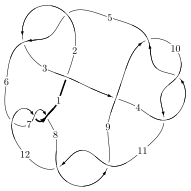
\includegraphics[width=112pt]{../../../GIT/diagram.site/Diagrams/png/1177_12a_0376.png}\\
\ \ \ A knot diagram\footnotemark}&
\allowdisplaybreaks
\textbf{Linearized knot diagam} \\
\cline{2-2}
 &
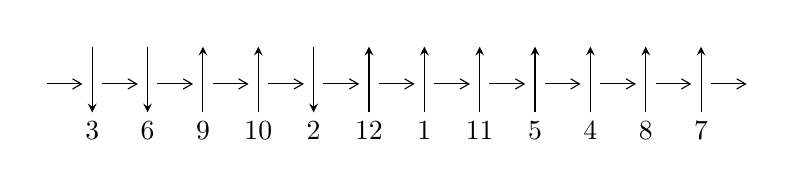
\begin{tikzpicture}[x=20pt, y=17pt]
	% nodes
	\node (C0) at (0, 0) {};
	\node (C1) at (1, 0) {};
	\node (C1U) at (1, +1) {};
	\node (C1D) at (1, -1) {3};

	\node (C2) at (2, 0) {};
	\node (C2U) at (2, +1) {};
	\node (C2D) at (2, -1) {6};

	\node (C3) at (3, 0) {};
	\node (C3U) at (3, +1) {};
	\node (C3D) at (3, -1) {9};

	\node (C4) at (4, 0) {};
	\node (C4U) at (4, +1) {};
	\node (C4D) at (4, -1) {10};

	\node (C5) at (5, 0) {};
	\node (C5U) at (5, +1) {};
	\node (C5D) at (5, -1) {2};

	\node (C6) at (6, 0) {};
	\node (C6U) at (6, +1) {};
	\node (C6D) at (6, -1) {12};

	\node (C7) at (7, 0) {};
	\node (C7U) at (7, +1) {};
	\node (C7D) at (7, -1) {1};

	\node (C8) at (8, 0) {};
	\node (C8U) at (8, +1) {};
	\node (C8D) at (8, -1) {11};

	\node (C9) at (9, 0) {};
	\node (C9U) at (9, +1) {};
	\node (C9D) at (9, -1) {5};

	\node (C10) at (10, 0) {};
	\node (C10U) at (10, +1) {};
	\node (C10D) at (10, -1) {4};

	\node (C11) at (11, 0) {};
	\node (C11U) at (11, +1) {};
	\node (C11D) at (11, -1) {8};

	\node (C12) at (12, 0) {};
	\node (C12U) at (12, +1) {};
	\node (C12D) at (12, -1) {7};
	\node (C13) at (13, 0) {};

	% arrows
	\draw[->,>={angle 60}]
	(C0) edge (C1) (C1) edge (C2) (C2) edge (C3) (C3) edge (C4) (C4) edge (C5) (C5) edge (C6) (C6) edge (C7) (C7) edge (C8) (C8) edge (C9) (C9) edge (C10) (C10) edge (C11) (C11) edge (C12) (C12) edge (C13) ;	\draw[->,>=stealth]
	(C1U) edge (C1D) (C2U) edge (C2D) (C3D) edge (C3U) (C4D) edge (C4U) (C5U) edge (C5D) (C6D) edge (C6U) (C7D) edge (C7U) (C8D) edge (C8U) (C9D) edge (C9U) (C10D) edge (C10U) (C11D) edge (C11U) (C12D) edge (C12U) ;
	\end{tikzpicture} \\
\hhline{~~} \\& 
\textbf{Solving Sequence} \\ \cline{2-2} 
 &
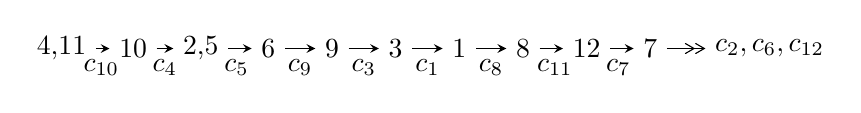
\begin{tikzpicture}[x=23pt, y=7pt]
	% node
	\node (A0) at (-1/8, 0) {4,11};
	\node (A1) at (1, 0) {10};
	\node (A2) at (33/16, 0) {2,5};
	\node (A3) at (25/8, 0) {6};
	\node (A4) at (33/8, 0) {9};
	\node (A5) at (41/8, 0) {3};
	\node (A6) at (49/8, 0) {1};
	\node (A7) at (57/8, 0) {8};
	\node (A8) at (65/8, 0) {12};
	\node (A9) at (73/8, 0) {7};
	\node (C1) at (1/2, -1) {$c_{10}$};
	\node (C2) at (3/2, -1) {$c_{4}$};
	\node (C3) at (21/8, -1) {$c_{5}$};
	\node (C4) at (29/8, -1) {$c_{9}$};
	\node (C5) at (37/8, -1) {$c_{3}$};
	\node (C6) at (45/8, -1) {$c_{1}$};
	\node (C7) at (53/8, -1) {$c_{8}$};
	\node (C8) at (61/8, -1) {$c_{11}$};
	\node (C9) at (69/8, -1) {$c_{7}$};
	\node (A10) at (11, 0) {$c_{2},c_{6},c_{12}$};

	% edge
	\draw[->,>=stealth]	
	(A0) edge (A1) (A1) edge (A2) (A2) edge (A3) (A3) edge (A4) (A4) edge (A5) (A5) edge (A6) (A6) edge (A7) (A7) edge (A8) (A8) edge (A9) ;
	\draw[->>,>={angle 60}]	
	(A9) edge (A10);
\end{tikzpicture} \\ 

\end{tabular} \\

\footnotetext{
The image of knot diagram is generated by the software ``\textbf{Draw programme}" developed by Andrew Bartholomew(\url{http://www.layer8.co.uk/maths/draw/index.htm\#Running-draw}), where we modified some parts for our purpose(\url{https://github.com/CATsTAILs/LinksPainter}).
}\phantom \\ \newline 
\centering \textbf{Ideals for irreducible components\footnotemark of $X_{\text{par}}$} 
 
\begin{align*}
I^u_{1}&=\langle 
- u^{46}-22 u^{44}+\cdots+4 b-4 u,\;u^{46}+21 u^{44}+\cdots+4 a+2,\;u^{49}-2 u^{48}+\cdots+4 u-2\rangle \\
I^u_{2}&=\langle 
-15 a^2 u^2-8 a^2 u+29 u^2 a-35 a^2+25 a u+26 u^2+22 b+86 a+8 u+46,\\
\phantom{I^u_{2}}&\phantom{= \langle  }a^3-4 u^2 a-2 a^2-5 a u- u^2+5 u-3,\;u^3+2 u-1\rangle \\
I^u_{3}&=\langle 
11 u^3 a^2-2 a^2 u^2+23 u^3 a+14 a^2 u-18 u^2 a-26 u^3+2 a^2+31 a u-16 u^2+19 b- a-40 u-22,\\
\phantom{I^u_{3}}&\phantom{= \langle  }a^3+2 a^2 u+u^2 a+2 a^2+5 a u+2 u^2- u-1,\;u^4+u^3+2 u^2+2 u+1\rangle \\
I^u_{4}&=\langle 
b- u+1,\;2 a+3 u-2,\;u^2+2\rangle \\
\\
I^v_{1}&=\langle 
a,\;b+1,\;v-1\rangle \\
\end{align*}
\raggedright * 5 irreducible components of $\dim_{\mathbb{C}}=0$, with total 73 representations.\\
\footnotetext{All coefficients of polynomials are rational numbers. But the coefficients are sometimes approximated in decimal forms when there is not enough margin.}
\newpage
\renewcommand{\arraystretch}{1}
\centering \section*{I. $I^u_{1}= \langle - u^{46}-22 u^{44}+\cdots+4 b-4 u,\;u^{46}+21 u^{44}+\cdots+4 a+2,\;u^{49}-2 u^{48}+\cdots+4 u-2 \rangle$}
\flushleft \textbf{(i) Arc colorings}\\
\begin{tabular}{m{7pt} m{180pt} m{7pt} m{180pt} }
\flushright $a_{4}=$&$\begin{pmatrix}0\\u\end{pmatrix}$ \\
\flushright $a_{11}=$&$\begin{pmatrix}1\\0\end{pmatrix}$ \\
\flushright $a_{10}=$&$\begin{pmatrix}1\\u^2\end{pmatrix}$ \\
\flushright $a_{2}=$&$\begin{pmatrix}-\frac{1}{4} u^{46}-\frac{21}{4} u^{44}+\cdots-\frac{1}{2} u-\frac{1}{2}\\\frac{1}{4} u^{46}+\frac{11}{2} u^{44}+\cdots+7 u^4+u\end{pmatrix}$ \\
\flushright $a_{5}=$&$\begin{pmatrix}u\\u^3+u\end{pmatrix}$ \\
\flushright $a_{6}=$&$\begin{pmatrix}-\frac{1}{2} u^{48}+u^{47}+\cdots+u-\frac{1}{2}\\u^{48}- u^{47}+\cdots-\frac{3}{2} u+1\end{pmatrix}$ \\
\flushright $a_{9}=$&$\begin{pmatrix}u^2+1\\u^4+2 u^2\end{pmatrix}$ \\
\flushright $a_{3}=$&$\begin{pmatrix}- u^5-2 u^3- u\\- u^7-3 u^5-2 u^3+u\end{pmatrix}$ \\
\flushright $a_{1}=$&$\begin{pmatrix}-\frac{1}{2} u^{48}+u^{47}+\cdots+2 u-\frac{3}{2}\\\frac{3}{4} u^{45}+\frac{63}{4} u^{43}+\cdots+\frac{1}{2} u-1\end{pmatrix}$ \\
\flushright $a_{8}=$&$\begin{pmatrix}- u^4- u^2+1\\u^4+2 u^2\end{pmatrix}$ \\
\flushright $a_{12}=$&$\begin{pmatrix}u^8+3 u^6+u^4-2 u^2+1\\- u^8-4 u^6-4 u^4\end{pmatrix}$ \\
\flushright $a_{7}=$&$\begin{pmatrix}-\frac{1}{4} u^{39}-\frac{9}{2} u^{37}+\cdots+\frac{1}{2} u+1\\-\frac{1}{4} u^{41}-\frac{19}{4} u^{39}+\cdots+\frac{5}{2} u^2+\frac{1}{2} u\end{pmatrix}$\\&\end{tabular}
\flushleft \textbf{(ii) Obstruction class $= -1$}\\~\\
\flushleft \textbf{(iii) Cusp Shapes $= 2 u^{48}-4 u^{47}+\cdots-2 u+8$}\\~\\
\newpage\renewcommand{\arraystretch}{1}
\flushleft \textbf{(iv) u-Polynomials at the component}\newline \\
\begin{tabular}{m{50pt}|m{274pt}}
Crossings & \hspace{64pt}u-Polynomials at each crossing \\
\hline $$\begin{aligned}c_{1}\end{aligned}$$&$\begin{aligned}
&u^{49}+26 u^{48}+\cdots+85 u+9
\end{aligned}$\\
\hline $$\begin{aligned}c_{2},c_{5}\end{aligned}$$&$\begin{aligned}
&u^{49}+2 u^{48}+\cdots-5 u-3
\end{aligned}$\\
\hline $$\begin{aligned}c_{3}\end{aligned}$$&$\begin{aligned}
&u^{49}+2 u^{48}+\cdots+796 u-202
\end{aligned}$\\
\hline $$\begin{aligned}c_{4},c_{9},c_{10}\end{aligned}$$&$\begin{aligned}
&u^{49}-2 u^{48}+\cdots+4 u-2
\end{aligned}$\\
\hline $$\begin{aligned}c_{6},c_{7},c_{12}\end{aligned}$$&$\begin{aligned}
&u^{49}-2 u^{48}+\cdots-9 u-3
\end{aligned}$\\
\hline $$\begin{aligned}c_{8},c_{11}\end{aligned}$$&$\begin{aligned}
&u^{49}+6 u^{48}+\cdots-672 u-144
\end{aligned}$\\
\hline
\end{tabular}\\~\\
\newpage\renewcommand{\arraystretch}{1}
\flushleft \textbf{(v) Riley Polynomials at the component}\newline \\
\begin{tabular}{m{50pt}|m{274pt}}
Crossings & \hspace{64pt}Riley Polynomials at each crossing \\
\hline $$\begin{aligned}c_{1}\end{aligned}$$&$\begin{aligned}
&y^{49}-2 y^{48}+\cdots+1321 y-81
\end{aligned}$\\
\hline $$\begin{aligned}c_{2},c_{5}\end{aligned}$$&$\begin{aligned}
&y^{49}-26 y^{48}+\cdots+85 y-9
\end{aligned}$\\
\hline $$\begin{aligned}c_{3}\end{aligned}$$&$\begin{aligned}
&y^{49}+22 y^{48}+\cdots-274576 y-40804
\end{aligned}$\\
\hline $$\begin{aligned}c_{4},c_{9},c_{10}\end{aligned}$$&$\begin{aligned}
&y^{49}+46 y^{48}+\cdots+8 y-4
\end{aligned}$\\
\hline $$\begin{aligned}c_{6},c_{7},c_{12}\end{aligned}$$&$\begin{aligned}
&y^{49}-42 y^{48}+\cdots-123 y-9
\end{aligned}$\\
\hline $$\begin{aligned}c_{8},c_{11}\end{aligned}$$&$\begin{aligned}
&y^{49}+42 y^{48}+\cdots-46080 y-20736
\end{aligned}$\\
\hline
\end{tabular}\\~\\
\newpage\flushleft \textbf{(vi) Complex Volumes and Cusp Shapes}
$$\begin{array}{c|c|c}  
\text{Solutions to }I^u_{1}& \I (\text{vol} + \sqrt{-1}CS) & \text{Cusp shape}\\
 \hline 
\begin{aligned}
u &= -0.167676 + 1.064370 I \\
a &= \phantom{-}0.778944 + 0.169238 I \\
b &= -0.470107 + 0.435995 I\end{aligned}
 & \phantom{-}3.40475 - 2.26424 I & \phantom{-}9.47951 + 3.87164 I \\ \hline\begin{aligned}
u &= -0.167676 - 1.064370 I \\
a &= \phantom{-}0.778944 - 0.169238 I \\
b &= -0.470107 - 0.435995 I\end{aligned}
 & \phantom{-}3.40475 + 2.26424 I & \phantom{-}9.47951 - 3.87164 I \\ \hline\begin{aligned}
u &= -0.617073 + 0.561498 I \\
a &= -1.89242 + 0.26973 I \\
b &= -0.37899 + 2.12914 I\end{aligned}
 & -2.80940 + 6.68744 I & \phantom{-}4.35067 - 3.31669 I \\ \hline\begin{aligned}
u &= -0.617073 - 0.561498 I \\
a &= -1.89242 - 0.26973 I \\
b &= -0.37899 - 2.12914 I\end{aligned}
 & -2.80940 - 6.68744 I & \phantom{-}4.35067 + 3.31669 I \\ \hline\begin{aligned}
u &= -0.715606 + 0.424836 I \\
a &= \phantom{-}1.350570 - 0.398846 I \\
b &= \phantom{-}0.62117 - 2.62903 I\end{aligned}
 & -2.31988 - 11.15510 I & \phantom{-}5.36635 + 8.72298 I \\ \hline\begin{aligned}
u &= -0.715606 - 0.424836 I \\
a &= \phantom{-}1.350570 + 0.398846 I \\
b &= \phantom{-}0.62117 + 2.62903 I\end{aligned}
 & -2.31988 + 11.15510 I & \phantom{-}5.36635 - 8.72298 I \\ \hline\begin{aligned}
u &= \phantom{-}0.677267 + 0.437562 I \\
a &= -1.279370 - 0.460443 I \\
b &= -0.40698 - 2.65012 I\end{aligned}
 & -6.72347 + 6.63996 I & \phantom{-}1.11534 - 6.53780 I \\ \hline\begin{aligned}
u &= \phantom{-}0.677267 - 0.437562 I \\
a &= -1.279370 + 0.460443 I \\
b &= -0.40698 + 2.65012 I\end{aligned}
 & -6.72347 - 6.63996 I & \phantom{-}1.11534 + 6.53780 I \\ \hline\begin{aligned}
u &= \phantom{-}0.252222 + 0.762976 I \\
a &= \phantom{-}0.970740 - 0.162669 I \\
b &= -0.393396 + 1.056380 I\end{aligned}
 & \phantom{-}3.14407 - 2.16679 I & \phantom{-}8.11057 + 2.63992 I \\ \hline\begin{aligned}
u &= \phantom{-}0.252222 - 0.762976 I \\
a &= \phantom{-}0.970740 + 0.162669 I \\
b &= -0.393396 - 1.056380 I\end{aligned}
 & \phantom{-}3.14407 + 2.16679 I & \phantom{-}8.11057 - 2.63992 I\\
 \hline 
 \end{array}$$\newpage$$\begin{array}{c|c|c}  
\text{Solutions to }I^u_{1}& \I (\text{vol} + \sqrt{-1}CS) & \text{Cusp shape}\\
 \hline 
\begin{aligned}
u &= \phantom{-}0.619485 + 0.505792 I \\
a &= \phantom{-}2.02337 + 0.19994 I \\
b &= \phantom{-}0.63493 + 2.03020 I\end{aligned}
 & -6.98732 - 2.33424 I & \phantom{-}0.197314 + 0.287759 I \\ \hline\begin{aligned}
u &= \phantom{-}0.619485 - 0.505792 I \\
a &= \phantom{-}2.02337 - 0.19994 I \\
b &= \phantom{-}0.63493 - 2.03020 I\end{aligned}
 & -6.98732 + 2.33424 I & \phantom{-}0.197314 - 0.287759 I \\ \hline\begin{aligned}
u &= \phantom{-}0.678594 + 0.396938 I \\
a &= -0.306907 - 0.562427 I \\
b &= \phantom{-}0.588764 - 0.054642 I\end{aligned}
 & \phantom{-}0.90488 + 6.19501 I & \phantom{-}8.65458 - 5.85948 I \\ \hline\begin{aligned}
u &= \phantom{-}0.678594 - 0.396938 I \\
a &= -0.306907 + 0.562427 I \\
b &= \phantom{-}0.588764 + 0.054642 I\end{aligned}
 & \phantom{-}0.90488 - 6.19501 I & \phantom{-}8.65458 + 5.85948 I \\ \hline\begin{aligned}
u &= \phantom{-}0.555271 + 0.515337 I \\
a &= -0.193065 - 0.411686 I \\
b &= \phantom{-}0.636055 + 0.278393 I\end{aligned}
 & \phantom{-}0.40390 - 2.07527 I & \phantom{-}7.58708 - 0.16558 I \\ \hline\begin{aligned}
u &= \phantom{-}0.555271 - 0.515337 I \\
a &= -0.193065 + 0.411686 I \\
b &= \phantom{-}0.636055 - 0.278393 I\end{aligned}
 & \phantom{-}0.40390 + 2.07527 I & \phantom{-}7.58708 + 0.16558 I \\ \hline\begin{aligned}
u &= \phantom{-}0.004497 + 1.254000 I \\
a &= -1.19737 - 0.79732 I \\
b &= \phantom{-}1.006470 + 0.945825 I\end{aligned}
 & -2.64701 + 1.46809 I & \phantom{-0.000000 } 0 \\ \hline\begin{aligned}
u &= \phantom{-}0.004497 - 1.254000 I \\
a &= -1.19737 + 0.79732 I \\
b &= \phantom{-}1.006470 - 0.945825 I\end{aligned}
 & -2.64701 - 1.46809 I & \phantom{-0.000000 } 0 \\ \hline\begin{aligned}
u &= \phantom{-}0.693958 + 0.185476 I \\
a &= -1.059550 + 0.036670 I \\
b &= -0.487962 - 1.323070 I\end{aligned}
 & \phantom{-}5.18309 + 5.73272 I & \phantom{-}11.27016 - 7.28979 I \\ \hline\begin{aligned}
u &= \phantom{-}0.693958 - 0.185476 I \\
a &= -1.059550 - 0.036670 I \\
b &= -0.487962 + 1.323070 I\end{aligned}
 & \phantom{-}5.18309 - 5.73272 I & \phantom{-}11.27016 + 7.28979 I\\
 \hline 
 \end{array}$$\newpage$$\begin{array}{c|c|c}  
\text{Solutions to }I^u_{1}& \I (\text{vol} + \sqrt{-1}CS) & \text{Cusp shape}\\
 \hline 
\begin{aligned}
u &= -0.233838 + 1.278280 I \\
a &= -0.114835 - 0.343745 I \\
b &= \phantom{-}0.465963 + 0.494287 I\end{aligned}
 & \phantom{-}2.08059 - 4.29919 I & \phantom{-0.000000 } 0 \\ \hline\begin{aligned}
u &= -0.233838 - 1.278280 I \\
a &= -0.114835 + 0.343745 I \\
b &= \phantom{-}0.465963 - 0.494287 I\end{aligned}
 & \phantom{-}2.08059 + 4.29919 I & \phantom{-0.000000 } 0 \\ \hline\begin{aligned}
u &= -0.670778 + 0.090636 I \\
a &= \phantom{-}0.695159 - 0.378048 I \\
b &= \phantom{-}0.035918 + 0.211766 I\end{aligned}
 & \phantom{-}6.30803 - 1.01693 I & \phantom{-}14.2364 + 0.8419 I \\ \hline\begin{aligned}
u &= -0.670778 - 0.090636 I \\
a &= \phantom{-}0.695159 + 0.378048 I \\
b &= \phantom{-}0.035918 - 0.211766 I\end{aligned}
 & \phantom{-}6.30803 + 1.01693 I & \phantom{-}14.2364 - 0.8419 I \\ \hline\begin{aligned}
u &= -0.196767 + 1.339410 I \\
a &= \phantom{-}1.98113 + 1.52913 I \\
b &= -0.93410 - 1.43004 I\end{aligned}
 & -4.92180 - 6.08417 I & \phantom{-0.000000 } 0 \\ \hline\begin{aligned}
u &= -0.196767 - 1.339410 I \\
a &= \phantom{-}1.98113 - 1.52913 I \\
b &= -0.93410 + 1.43004 I\end{aligned}
 & -4.92180 + 6.08417 I & \phantom{-0.000000 } 0 \\ \hline\begin{aligned}
u &= \phantom{-}0.265708 + 1.335960 I \\
a &= -1.24758 + 1.71469 I \\
b &= -0.054082 - 1.297110 I\end{aligned}
 & \phantom{-}0.40943 + 9.20745 I & \phantom{-0.000000 } 0 \\ \hline\begin{aligned}
u &= \phantom{-}0.265708 - 1.335960 I \\
a &= -1.24758 - 1.71469 I \\
b &= -0.054082 + 1.297110 I\end{aligned}
 & \phantom{-}0.40943 - 9.20745 I & \phantom{-0.000000 } 0 \\ \hline\begin{aligned}
u &= -0.565566 + 0.178039 I \\
a &= \phantom{-}0.847644 - 0.080313 I \\
b &= -0.168017 - 1.386940 I\end{aligned}
 & -0.16483 - 3.30304 I & \phantom{-}6.58993 + 8.73893 I \\ \hline\begin{aligned}
u &= -0.565566 - 0.178039 I \\
a &= \phantom{-}0.847644 + 0.080313 I \\
b &= -0.168017 + 1.386940 I\end{aligned}
 & -0.16483 + 3.30304 I & \phantom{-}6.58993 - 8.73893 I\\
 \hline 
 \end{array}$$\newpage$$\begin{array}{c|c|c}  
\text{Solutions to }I^u_{1}& \I (\text{vol} + \sqrt{-1}CS) & \text{Cusp shape}\\
 \hline 
\begin{aligned}
u &= -0.075529 + 1.409520 I \\
a &= -0.06668 - 2.20376 I \\
b &= -0.56477 + 1.41957 I\end{aligned}
 & -7.18390 - 0.26810 I & \phantom{-0.000000 } 0 \\ \hline\begin{aligned}
u &= -0.075529 - 1.409520 I \\
a &= -0.06668 + 2.20376 I \\
b &= -0.56477 - 1.41957 I\end{aligned}
 & -7.18390 + 0.26810 I & \phantom{-0.000000 } 0 \\ \hline\begin{aligned}
u &= \phantom{-}0.25245 + 1.46110 I \\
a &= -0.594045 - 0.560678 I \\
b &= \phantom{-}0.440686 + 0.137021 I\end{aligned}
 & -5.08167 + 9.59602 I & \phantom{-0.000000 } 0 \\ \hline\begin{aligned}
u &= \phantom{-}0.25245 - 1.46110 I \\
a &= -0.594045 + 0.560678 I \\
b &= \phantom{-}0.440686 - 0.137021 I\end{aligned}
 & -5.08167 - 9.59602 I & \phantom{-0.000000 } 0 \\ \hline\begin{aligned}
u &= \phantom{-}0.19236 + 1.47058 I \\
a &= -0.541758 - 0.828898 I \\
b &= \phantom{-}0.550975 + 0.570094 I\end{aligned}
 & -5.96591 + 0.62329 I & \phantom{-0.000000 } 0 \\ \hline\begin{aligned}
u &= \phantom{-}0.19236 - 1.47058 I \\
a &= -0.541758 + 0.828898 I \\
b &= \phantom{-}0.550975 - 0.570094 I\end{aligned}
 & -5.96591 - 0.62329 I & \phantom{-0.000000 } 0 \\ \hline\begin{aligned}
u &= \phantom{-}0.04361 + 1.49144 I \\
a &= \phantom{-}0.26431 - 2.05562 I \\
b &= \phantom{-}0.16481 + 1.98787 I\end{aligned}
 & -3.91948 - 1.38659 I & \phantom{-0.000000 } 0 \\ \hline\begin{aligned}
u &= \phantom{-}0.04361 - 1.49144 I \\
a &= \phantom{-}0.26431 + 2.05562 I \\
b &= \phantom{-}0.16481 - 1.98787 I\end{aligned}
 & -3.91948 + 1.38659 I & \phantom{-0.000000 } 0 \\ \hline\begin{aligned}
u &= \phantom{-}0.24647 + 1.47591 I \\
a &= -1.23308 + 3.23255 I \\
b &= -0.78225 - 3.64550 I\end{aligned}
 & -12.9040 + 10.0134 I & \phantom{-0.000000 } 0 \\ \hline\begin{aligned}
u &= \phantom{-}0.24647 - 1.47591 I \\
a &= -1.23308 - 3.23255 I \\
b &= -0.78225 + 3.64550 I\end{aligned}
 & -12.9040 - 10.0134 I & \phantom{-0.000000 } 0\\
 \hline 
 \end{array}$$\newpage$$\begin{array}{c|c|c}  
\text{Solutions to }I^u_{1}& \I (\text{vol} + \sqrt{-1}CS) & \text{Cusp shape}\\
 \hline 
\begin{aligned}
u &= -0.26382 + 1.47698 I \\
a &= \phantom{-}1.05482 + 3.15508 I \\
b &= \phantom{-}1.08638 - 3.45807 I\end{aligned}
 & -8.4594 - 14.7285 I & \phantom{-0.000000 } 0 \\ \hline\begin{aligned}
u &= -0.26382 - 1.47698 I \\
a &= \phantom{-}1.05482 - 3.15508 I \\
b &= \phantom{-}1.08638 + 3.45807 I\end{aligned}
 & -8.4594 + 14.7285 I & \phantom{-0.000000 } 0 \\ \hline\begin{aligned}
u &= \phantom{-}0.21115 + 1.48782 I \\
a &= \phantom{-}0.15274 - 2.56686 I \\
b &= \phantom{-}1.82838 + 2.31454 I\end{aligned}
 & -13.44400 + 0.67957 I & \phantom{-0.000000 } 0 \\ \hline\begin{aligned}
u &= \phantom{-}0.21115 - 1.48782 I \\
a &= \phantom{-}0.15274 + 2.56686 I \\
b &= \phantom{-}1.82838 - 2.31454 I\end{aligned}
 & -13.44400 - 0.67957 I & \phantom{-0.000000 } 0 \\ \hline\begin{aligned}
u &= -0.19310 + 1.50554 I \\
a &= -0.22564 - 2.54437 I \\
b &= -1.59683 + 2.50677 I\end{aligned}
 & -9.54977 + 3.78347 I & \phantom{-0.000000 } 0 \\ \hline\begin{aligned}
u &= -0.19310 - 1.50554 I \\
a &= -0.22564 + 2.54437 I \\
b &= -1.59683 - 2.50677 I\end{aligned}
 & -9.54977 - 3.78347 I & \phantom{-0.000000 } 0 \\ \hline\begin{aligned}
u &= -0.202679 + 0.413695 I \\
a &= -1.41900 - 1.17309 I \\
b &= -0.167114 + 0.794243 I\end{aligned}
 & -1.52088 + 0.82300 I & -1.75933 - 1.01274 I \\ \hline\begin{aligned}
u &= -0.202679 - 0.413695 I \\
a &= -1.41900 + 1.17309 I \\
b &= -0.167114 - 0.794243 I\end{aligned}
 & -1.52088 - 0.82300 I & -1.75933 + 1.01274 I \\ \hline\begin{aligned}
u &= \phantom{-}0.418775\phantom{ +0.000000I} \\
a &= -0.496253\phantom{ +0.000000I} \\
b &= \phantom{-}0.688205\phantom{ +0.000000I}\end{aligned}
 & \phantom{-}0.773938\phantom{ +0.000000I} & \phantom{-}13.3940\phantom{ +0.000000I}\\
 \hline 
 \end{array}$$\newpage\newpage\renewcommand{\arraystretch}{1}
\centering \section*{II. $I^u_{2}= \langle -15 a^2 u^2+29 u^2 a+\cdots+86 a+46,\;a^3-4 u^2 a-2 a^2-5 a u- u^2+5 u-3,\;u^3+2 u-1 \rangle$}
\flushleft \textbf{(i) Arc colorings}\\
\begin{tabular}{m{7pt} m{180pt} m{7pt} m{180pt} }
\flushright $a_{4}=$&$\begin{pmatrix}0\\u\end{pmatrix}$ \\
\flushright $a_{11}=$&$\begin{pmatrix}1\\0\end{pmatrix}$ \\
\flushright $a_{10}=$&$\begin{pmatrix}1\\u^2\end{pmatrix}$ \\
\flushright $a_{2}=$&$\begin{pmatrix}a\\0.681818 a^{2} u^{2}-1.31818 a u^{2}+\cdots-3.90909 a-2.09091\end{pmatrix}$ \\
\flushright $a_{5}=$&$\begin{pmatrix}u\\- u+1\end{pmatrix}$ \\
\flushright $a_{6}=$&$\begin{pmatrix}-0.409091 a^{2} u^{2}+0.590909 a u^{2}+\cdots+1.54545 a+0.454545\\\frac{1}{2} a^2 u^2-\frac{3}{2} u^2 a+\cdots-4 a-1\end{pmatrix}$ \\
\flushright $a_{9}=$&$\begin{pmatrix}u^2+1\\u\end{pmatrix}$ \\
\flushright $a_{3}=$&$\begin{pmatrix}- u^2- u\\u^2\end{pmatrix}$ \\
\flushright $a_{1}=$&$\begin{pmatrix}0.0454545 a^{2} u^{2}+0.0454545 a u^{2}+\cdots-0.727273 a-0.272727\\0.818182 a^{2} u^{2}-1.68182 a u^{2}+\cdots-3.59091 a-1.90909\end{pmatrix}$ \\
\flushright $a_{8}=$&$\begin{pmatrix}u^2- u+1\\u\end{pmatrix}$ \\
\flushright $a_{12}=$&$\begin{pmatrix}u^2+u\\- u^2\end{pmatrix}$ \\
\flushright $a_{7}=$&$\begin{pmatrix}-0.227273 a^{2} u^{2}+0.272727 a u^{2}+\cdots+0.136364 a+0.363636\\0.545455 a^{2} u^{2}-1.45455 a u^{2}+\cdots-3.72727 a-1.27273\end{pmatrix}$\\&\end{tabular}
\flushleft \textbf{(ii) Obstruction class $= -1$}\\~\\
\flushleft \textbf{(iii) Cusp Shapes $= 4 u^2+4 u+10$}\\~\\
\newpage\renewcommand{\arraystretch}{1}
\flushleft \textbf{(iv) u-Polynomials at the component}\newline \\
\begin{tabular}{m{50pt}|m{274pt}}
Crossings & \hspace{64pt}u-Polynomials at each crossing \\
\hline $$\begin{aligned}c_{1}\end{aligned}$$&$\begin{aligned}
&u^9+6 u^8+15 u^7+16 u^6- u^5-18 u^4-11 u^3+4 u^2+4 u+1
\end{aligned}$\\
\hline $$\begin{aligned}c_{2},c_{5},c_{6}\\c_{7},c_{12}\end{aligned}$$&$\begin{aligned}
&u^9-3 u^7+3 u^5+u^3-2 u+1
\end{aligned}$\\
\hline $$\begin{aligned}c_{3}\end{aligned}$$&$\begin{aligned}
&(u^3-3 u^2+5 u-2)^3
\end{aligned}$\\
\hline $$\begin{aligned}c_{4},c_{8},c_{9}\\c_{10},c_{11}\end{aligned}$$&$\begin{aligned}
&(u^3+2 u-1)^3
\end{aligned}$\\
\hline
\end{tabular}\\~\\
\newpage\renewcommand{\arraystretch}{1}
\flushleft \textbf{(v) Riley Polynomials at the component}\newline \\
\begin{tabular}{m{50pt}|m{274pt}}
Crossings & \hspace{64pt}Riley Polynomials at each crossing \\
\hline $$\begin{aligned}c_{1}\end{aligned}$$&$\begin{aligned}
&y^9-6 y^8+31 y^7-92 y^6+207 y^5-322 y^4+225 y^3-68 y^2+8 y-1
\end{aligned}$\\
\hline $$\begin{aligned}c_{2},c_{5},c_{6}\\c_{7},c_{12}\end{aligned}$$&$\begin{aligned}
&y^9-6 y^8+15 y^7-16 y^6- y^5+18 y^4-11 y^3-4 y^2+4 y-1
\end{aligned}$\\
\hline $$\begin{aligned}c_{3}\end{aligned}$$&$\begin{aligned}
&(y^3+y^2+13 y-4)^3
\end{aligned}$\\
\hline $$\begin{aligned}c_{4},c_{8},c_{9}\\c_{10},c_{11}\end{aligned}$$&$\begin{aligned}
&(y^3+4 y^2+4 y-1)^3
\end{aligned}$\\
\hline
\end{tabular}\\~\\
\newpage\flushleft \textbf{(vi) Complex Volumes and Cusp Shapes}
$$\begin{array}{c|c|c}  
\text{Solutions to }I^u_{2}& \I (\text{vol} + \sqrt{-1}CS) & \text{Cusp shape}\\
 \hline 
\begin{aligned}
u &= -0.22670 + 1.46771 I \\
a &= \phantom{-}0.583843 - 0.678582 I \\
b &= -0.519013 + 0.319210 I\end{aligned}
 & -9.44074 - 5.13794 I & \phantom{-}0.68207 + 3.20902 I \\ \hline\begin{aligned}
u &= -0.22670 + 1.46771 I \\
a &= -0.07989 - 2.57481 I \\
b &= -2.01693 + 2.08171 I\end{aligned}
 & -9.44074 - 5.13794 I & \phantom{-}0.68207 + 3.20902 I \\ \hline\begin{aligned}
u &= -0.22670 + 1.46771 I \\
a &= \phantom{-}1.49604 + 3.25339 I \\
b &= \phantom{-}0.33038 - 3.73184 I\end{aligned}
 & -9.44074 - 5.13794 I & \phantom{-}0.68207 + 3.20902 I \\ \hline\begin{aligned}
u &= -0.22670 - 1.46771 I \\
a &= \phantom{-}0.583843 + 0.678582 I \\
b &= -0.519013 - 0.319210 I\end{aligned}
 & -9.44074 + 5.13794 I & \phantom{-}0.68207 - 3.20902 I \\ \hline\begin{aligned}
u &= -0.22670 - 1.46771 I \\
a &= -0.07989 + 2.57481 I \\
b &= -2.01693 - 2.08171 I\end{aligned}
 & -9.44074 + 5.13794 I & \phantom{-}0.68207 - 3.20902 I \\ \hline\begin{aligned}
u &= -0.22670 - 1.46771 I \\
a &= \phantom{-}1.49604 - 3.25339 I \\
b &= \phantom{-}0.33038 + 3.73184 I\end{aligned}
 & -9.44074 + 5.13794 I & \phantom{-}0.68207 - 3.20902 I \\ \hline\begin{aligned}
u &= \phantom{-}0.453398\phantom{ +0.000000I} \\
a &= -0.547908 + 0.054538 I \\
b &= \phantom{-}0.637390 - 0.369377 I\end{aligned}
 & \phantom{-}0.787199\phantom{ +0.000000I} & \phantom{-}12.6360\phantom{ +0.000000I} \\ \hline\begin{aligned}
u &= \phantom{-}0.453398\phantom{ +0.000000I} \\
a &= -0.547908 - 0.054538 I \\
b &= \phantom{-}0.637390 + 0.369377 I\end{aligned}
 & \phantom{-}0.787199\phantom{ +0.000000I} & \phantom{-}12.6360\phantom{ +0.000000I} \\ \hline\begin{aligned}
u &= \phantom{-}0.453398\phantom{ +0.000000I} \\
a &= \phantom{-}3.09582\phantom{ +0.000000I} \\
b &= \phantom{-}1.13636\phantom{ +0.000000I}\end{aligned}
 & \phantom{-}0.787199\phantom{ +0.000000I} & \phantom{-}12.6360\phantom{ +0.000000I}\\
 \hline 
 \end{array}$$\newpage\newpage\renewcommand{\arraystretch}{1}
\centering \section*{III. $I^u_{3}= \langle 11 u^3 a^2+23 u^3 a+\cdots- a-22,\;a^3+2 a^2 u+u^2 a+2 a^2+5 a u+2 u^2- u-1,\;u^4+u^3+2 u^2+2 u+1 \rangle$}
\flushleft \textbf{(i) Arc colorings}\\
\begin{tabular}{m{7pt} m{180pt} m{7pt} m{180pt} }
\flushright $a_{4}=$&$\begin{pmatrix}0\\u\end{pmatrix}$ \\
\flushright $a_{11}=$&$\begin{pmatrix}1\\0\end{pmatrix}$ \\
\flushright $a_{10}=$&$\begin{pmatrix}1\\u^2\end{pmatrix}$ \\
\flushright $a_{2}=$&$\begin{pmatrix}a\\-0.578947 a^{2} u^{3}-1.21053 a u^{3}+\cdots+0.0526316 a+1.15789\end{pmatrix}$ \\
\flushright $a_{5}=$&$\begin{pmatrix}u\\u^3+u\end{pmatrix}$ \\
\flushright $a_{6}=$&$\begin{pmatrix}0.315789 a^{2} u^{3}+0.842105 a u^{3}+\cdots+1.78947 a-0.631579\\-0.947368 a^{2} u^{3}-0.526316 a u^{3}+\cdots+0.631579 a+1.89474\end{pmatrix}$ \\
\flushright $a_{9}=$&$\begin{pmatrix}u^2+1\\- u^3-2 u-1\end{pmatrix}$ \\
\flushright $a_{3}=$&$\begin{pmatrix}- u^3-2 u-1\\- u^3- u^2- u-2\end{pmatrix}$ \\
\flushright $a_{1}=$&$\begin{pmatrix}0.789474 a^{2} u^{3}+0.105263 a u^{3}+\cdots-0.526316 a-1.57895\\0.789474 a^{2} u^{3}+1.10526 a u^{3}+\cdots+2.47368 a-1.57895\end{pmatrix}$ \\
\flushright $a_{8}=$&$\begin{pmatrix}u^3+u^2+2 u+2\\- u^3-2 u-1\end{pmatrix}$ \\
\flushright $a_{12}=$&$\begin{pmatrix}u^3+2 u+1\\u^3+u^2+u+2\end{pmatrix}$ \\
\flushright $a_{7}=$&$\begin{pmatrix}0.263158 a^{2} u^{3}+1.36842 a u^{3}+\cdots+1.15789 a-0.526316\\-0.105263 a^{2} u^{3}+1.05263 a u^{3}+\cdots+2.73684 a+0.210526\end{pmatrix}$\\&\end{tabular}
\flushleft \textbf{(ii) Obstruction class $= -1$}\\~\\
\flushleft \textbf{(iii) Cusp Shapes $= 4 u^3+4 u+6$}\\~\\
\newpage\renewcommand{\arraystretch}{1}
\flushleft \textbf{(iv) u-Polynomials at the component}\newline \\
\begin{tabular}{m{50pt}|m{274pt}}
Crossings & \hspace{64pt}u-Polynomials at each crossing \\
\hline $$\begin{aligned}c_{1}\end{aligned}$$&$\begin{aligned}
&u^{12}+8 u^{11}+\cdots+2 u^2+1
\end{aligned}$\\
\hline $$\begin{aligned}c_{2},c_{5},c_{6}\\c_{7},c_{12}\end{aligned}$$&$\begin{aligned}
&u^{12}-4 u^{10}- u^9+6 u^8+3 u^7-2 u^6-3 u^5-3 u^4- u^3+2 u^2+2 u+1
\end{aligned}$\\
\hline $$\begin{aligned}c_{3}\end{aligned}$$&$\begin{aligned}
&(u^2+u+1)^6
\end{aligned}$\\
\hline $$\begin{aligned}c_{4},c_{8},c_{9}\\c_{10},c_{11}\end{aligned}$$&$\begin{aligned}
&(u^4+u^3+2 u^2+2 u+1)^3
\end{aligned}$\\
\hline
\end{tabular}\\~\\
\newpage\renewcommand{\arraystretch}{1}
\flushleft \textbf{(v) Riley Polynomials at the component}\newline \\
\begin{tabular}{m{50pt}|m{274pt}}
Crossings & \hspace{64pt}Riley Polynomials at each crossing \\
\hline $$\begin{aligned}c_{1}\end{aligned}$$&$\begin{aligned}
&y^{12}-8 y^{11}+\cdots+4 y+1
\end{aligned}$\\
\hline $$\begin{aligned}c_{2},c_{5},c_{6}\\c_{7},c_{12}\end{aligned}$$&$\begin{aligned}
&y^{12}-8 y^{11}+\cdots+2 y^2+1
\end{aligned}$\\
\hline $$\begin{aligned}c_{3}\end{aligned}$$&$\begin{aligned}
&(y^2+y+1)^6
\end{aligned}$\\
\hline $$\begin{aligned}c_{4},c_{8},c_{9}\\c_{10},c_{11}\end{aligned}$$&$\begin{aligned}
&(y^4+3 y^3+2 y^2+1)^3
\end{aligned}$\\
\hline
\end{tabular}\\~\\
\newpage\flushleft \textbf{(vi) Complex Volumes and Cusp Shapes}
$$\begin{array}{c|c|c}  
\text{Solutions to }I^u_{3}& \I (\text{vol} + \sqrt{-1}CS) & \text{Cusp shape}\\
 \hline 
\begin{aligned}
u &= -0.621744 + 0.440597 I \\
a &= \phantom{-}1.164420 - 0.511133 I \\
b &= \phantom{-}0.14782 - 2.60434 I\end{aligned}
 & -3.28987 - 2.02988 I & \phantom{-}4.00000 + 3.46410 I \\ \hline\begin{aligned}
u &= -0.621744 + 0.440597 I \\
a &= \phantom{-}0.253508 - 0.493412 I \\
b &= -0.619418 + 0.097186 I\end{aligned}
 & -3.28987 - 2.02988 I & \phantom{-}4.00000 + 3.46410 I \\ \hline\begin{aligned}
u &= -0.621744 + 0.440597 I \\
a &= -2.17444 + 0.12335 I \\
b &= -0.91328 + 1.87086 I\end{aligned}
 & -3.28987 - 2.02988 I & \phantom{-}4.00000 + 3.46410 I \\ \hline\begin{aligned}
u &= -0.621744 - 0.440597 I \\
a &= \phantom{-}1.164420 + 0.511133 I \\
b &= \phantom{-}0.14782 + 2.60434 I\end{aligned}
 & -3.28987 + 2.02988 I & \phantom{-}4.00000 - 3.46410 I \\ \hline\begin{aligned}
u &= -0.621744 - 0.440597 I \\
a &= \phantom{-}0.253508 + 0.493412 I \\
b &= -0.619418 - 0.097186 I\end{aligned}
 & -3.28987 + 2.02988 I & \phantom{-}4.00000 - 3.46410 I \\ \hline\begin{aligned}
u &= -0.621744 - 0.440597 I \\
a &= -2.17444 - 0.12335 I \\
b &= -0.91328 - 1.87086 I\end{aligned}
 & -3.28987 + 2.02988 I & \phantom{-}4.00000 - 3.46410 I \\ \hline\begin{aligned}
u &= \phantom{-}0.121744 + 1.306620 I \\
a &= \phantom{-}0.276849 - 0.783184 I \\
b &= -0.361992 + 0.876949 I\end{aligned}
 & -3.28987 + 2.02988 I & \phantom{-}4.00000 - 3.46410 I \\ \hline\begin{aligned}
u &= \phantom{-}0.121744 + 1.306620 I \\
a &= -0.07790 - 2.21669 I \\
b &= \phantom{-}0.939408 + 0.575735 I\end{aligned}
 & -3.28987 + 2.02988 I & \phantom{-}4.00000 - 3.46410 I \\ \hline\begin{aligned}
u &= \phantom{-}0.121744 + 1.306620 I \\
a &= -2.44244 + 0.38663 I \\
b &= \phantom{-}1.80746 - 0.35693 I\end{aligned}
 & -3.28987 + 2.02988 I & \phantom{-}4.00000 - 3.46410 I \\ \hline\begin{aligned}
u &= \phantom{-}0.121744 - 1.306620 I \\
a &= \phantom{-}0.276849 + 0.783184 I \\
b &= -0.361992 - 0.876949 I\end{aligned}
 & -3.28987 - 2.02988 I & \phantom{-}4.00000 + 3.46410 I\\
 \hline 
 \end{array}$$\newpage$$\begin{array}{c|c|c}  
\text{Solutions to }I^u_{3}& \I (\text{vol} + \sqrt{-1}CS) & \text{Cusp shape}\\
 \hline 
\begin{aligned}
u &= \phantom{-}0.121744 - 1.306620 I \\
a &= -0.07790 + 2.21669 I \\
b &= \phantom{-}0.939408 - 0.575735 I\end{aligned}
 & -3.28987 - 2.02988 I & \phantom{-}4.00000 + 3.46410 I \\ \hline\begin{aligned}
u &= \phantom{-}0.121744 - 1.306620 I \\
a &= -2.44244 - 0.38663 I \\
b &= \phantom{-}1.80746 + 0.35693 I\end{aligned}
 & -3.28987 - 2.02988 I & \phantom{-}4.00000 + 3.46410 I\\
 \hline 
 \end{array}$$\newpage\newpage\renewcommand{\arraystretch}{1}
\centering \section*{IV. $I^u_{4}= \langle b- u+1,\;2 a+3 u-2,\;u^2+2 \rangle$}
\flushleft \textbf{(i) Arc colorings}\\
\begin{tabular}{m{7pt} m{180pt} m{7pt} m{180pt} }
\flushright $a_{4}=$&$\begin{pmatrix}0\\u\end{pmatrix}$ \\
\flushright $a_{11}=$&$\begin{pmatrix}1\\0\end{pmatrix}$ \\
\flushright $a_{10}=$&$\begin{pmatrix}1\\-2\end{pmatrix}$ \\
\flushright $a_{2}=$&$\begin{pmatrix}-\frac{3}{2} u+1\\u-1\end{pmatrix}$ \\
\flushright $a_{5}=$&$\begin{pmatrix}u\\- u\end{pmatrix}$ \\
\flushright $a_{6}=$&$\begin{pmatrix}-\frac{1}{2} u+1\\-1\end{pmatrix}$ \\
\flushright $a_{9}=$&$\begin{pmatrix}-1\\0\end{pmatrix}$ \\
\flushright $a_{3}=$&$\begin{pmatrix}- u\\u\end{pmatrix}$ \\
\flushright $a_{1}=$&$\begin{pmatrix}-\frac{1}{2} u+1\\-1\end{pmatrix}$ \\
\flushright $a_{8}=$&$\begin{pmatrix}-1\\0\end{pmatrix}$ \\
\flushright $a_{12}=$&$\begin{pmatrix}1\\0\end{pmatrix}$ \\
\flushright $a_{7}=$&$\begin{pmatrix}-\frac{1}{2} u\\-1\end{pmatrix}$\\&\end{tabular}
\flushleft \textbf{(ii) Obstruction class $= 1$}\\~\\
\flushleft \textbf{(iii) Cusp Shapes $= 0$}\\~\\
\newpage\renewcommand{\arraystretch}{1}
\flushleft \textbf{(iv) u-Polynomials at the component}\newline \\
\begin{tabular}{m{50pt}|m{274pt}}
Crossings & \hspace{64pt}u-Polynomials at each crossing \\
\hline $$\begin{aligned}c_{1},c_{5},c_{6}\\c_{7}\end{aligned}$$&$\begin{aligned}
&(u-1)^2
\end{aligned}$\\
\hline $$\begin{aligned}c_{2},c_{12}\end{aligned}$$&$\begin{aligned}
&(u+1)^2
\end{aligned}$\\
\hline $$\begin{aligned}c_{3},c_{4},c_{9}\\c_{10}\end{aligned}$$&$\begin{aligned}
&u^2+2
\end{aligned}$\\
\hline $$\begin{aligned}c_{8},c_{11}\end{aligned}$$&$\begin{aligned}
&u^2
\end{aligned}$\\
\hline
\end{tabular}\\~\\
\newpage\renewcommand{\arraystretch}{1}
\flushleft \textbf{(v) Riley Polynomials at the component}\newline \\
\begin{tabular}{m{50pt}|m{274pt}}
Crossings & \hspace{64pt}Riley Polynomials at each crossing \\
\hline $$\begin{aligned}c_{1},c_{2},c_{5}\\c_{6},c_{7},c_{12}\end{aligned}$$&$\begin{aligned}
&(y-1)^2
\end{aligned}$\\
\hline $$\begin{aligned}c_{3},c_{4},c_{9}\\c_{10}\end{aligned}$$&$\begin{aligned}
&(y+2)^2
\end{aligned}$\\
\hline $$\begin{aligned}c_{8},c_{11}\end{aligned}$$&$\begin{aligned}
&y^2
\end{aligned}$\\
\hline
\end{tabular}\\~\\
\newpage\flushleft \textbf{(vi) Complex Volumes and Cusp Shapes}
$$\begin{array}{c|c|c}  
\text{Solutions to }I^u_{4}& \I (\text{vol} + \sqrt{-1}CS) & \text{Cusp shape}\\
 \hline 
\begin{aligned}
u &= \phantom{-0.000000 -}1.414210 I \\
a &= \phantom{-}1.00000 - 2.12132 I \\
b &= -1.00000 + 1.41421 I\end{aligned}
 & -4.93480\phantom{ +0.000000I} & \phantom{-0.000000 } 0 \\ \hline\begin{aligned}
u &= \phantom{-0.000000 } -1.414210 I \\
a &= \phantom{-}1.00000 + 2.12132 I \\
b &= -1.00000 - 1.41421 I\end{aligned}
 & -4.93480\phantom{ +0.000000I} & \phantom{-0.000000 } 0\\
 \hline 
 \end{array}$$\newpage\newpage\renewcommand{\arraystretch}{1}
\centering \section*{V. $I^v_{1}= \langle a,\;b+1,\;v-1 \rangle$}
\flushleft \textbf{(i) Arc colorings}\\
\begin{tabular}{m{7pt} m{180pt} m{7pt} m{180pt} }
\flushright $a_{4}=$&$\begin{pmatrix}1\\0\end{pmatrix}$ \\
\flushright $a_{11}=$&$\begin{pmatrix}1\\0\end{pmatrix}$ \\
\flushright $a_{10}=$&$\begin{pmatrix}1\\0\end{pmatrix}$ \\
\flushright $a_{2}=$&$\begin{pmatrix}0\\-1\end{pmatrix}$ \\
\flushright $a_{5}=$&$\begin{pmatrix}1\\0\end{pmatrix}$ \\
\flushright $a_{6}=$&$\begin{pmatrix}1\\1\end{pmatrix}$ \\
\flushright $a_{9}=$&$\begin{pmatrix}1\\0\end{pmatrix}$ \\
\flushright $a_{3}=$&$\begin{pmatrix}1\\0\end{pmatrix}$ \\
\flushright $a_{1}=$&$\begin{pmatrix}-1\\-1\end{pmatrix}$ \\
\flushright $a_{8}=$&$\begin{pmatrix}1\\0\end{pmatrix}$ \\
\flushright $a_{12}=$&$\begin{pmatrix}1\\0\end{pmatrix}$ \\
\flushright $a_{7}=$&$\begin{pmatrix}2\\1\end{pmatrix}$\\&\end{tabular}
\flushleft \textbf{(ii) Obstruction class $= 1$}\\~\\
\flushleft \textbf{(iii) Cusp Shapes $= 0$}\\~\\
\newpage\renewcommand{\arraystretch}{1}
\flushleft \textbf{(iv) u-Polynomials at the component}\newline \\
\begin{tabular}{m{50pt}|m{274pt}}
Crossings & \hspace{64pt}u-Polynomials at each crossing \\
\hline $$\begin{aligned}c_{1},c_{2},c_{12}\end{aligned}$$&$\begin{aligned}
&u-1
\end{aligned}$\\
\hline $$\begin{aligned}c_{3},c_{4},c_{8}\\c_{9},c_{10},c_{11}\end{aligned}$$&$\begin{aligned}
&u
\end{aligned}$\\
\hline $$\begin{aligned}c_{5},c_{6},c_{7}\end{aligned}$$&$\begin{aligned}
&u+1
\end{aligned}$\\
\hline
\end{tabular}\\~\\
\newpage\renewcommand{\arraystretch}{1}
\flushleft \textbf{(v) Riley Polynomials at the component}\newline \\
\begin{tabular}{m{50pt}|m{274pt}}
Crossings & \hspace{64pt}Riley Polynomials at each crossing \\
\hline $$\begin{aligned}c_{1},c_{2},c_{5}\\c_{6},c_{7},c_{12}\end{aligned}$$&$\begin{aligned}
&y-1
\end{aligned}$\\
\hline $$\begin{aligned}c_{3},c_{4},c_{8}\\c_{9},c_{10},c_{11}\end{aligned}$$&$\begin{aligned}
&y
\end{aligned}$\\
\hline
\end{tabular}\\~\\
\newpage\flushleft \textbf{(vi) Complex Volumes and Cusp Shapes}
$$\begin{array}{c|c|c}  
\text{Solutions to }I^v_{1}& \I (\text{vol} + \sqrt{-1}CS) & \text{Cusp shape}\\
 \hline 
\begin{aligned}
v &= \phantom{-}1.00000\phantom{ +0.000000I} \\
a &= \phantom{-0.000000 } 0 \\
b &= -1.00000\phantom{ +0.000000I}\end{aligned}
 & \phantom{-0.000000 } 0 & \phantom{-0.000000 } 0\\
 \hline 
 \end{array}$$\newpage
\newpage\renewcommand{\arraystretch}{1}
\centering \section*{ VI. u-Polynomials}
\begin{tabular}{m{50pt}|m{274pt}}
Crossings & \hspace{64pt}u-Polynomials at each crossing \\
\hline $$\begin{aligned}c_{1}\end{aligned}$$&$\begin{aligned}
&((u-1)^3)(u^9+6 u^8+\cdots+4 u+1)\\
&\cdot(u^{12}+8 u^{11}+\cdots+2 u^2+1)(u^{49}+26 u^{48}+\cdots+85 u+9)
\end{aligned}$\\
\hline $$\begin{aligned}c_{2}\end{aligned}$$&$\begin{aligned}
&(u-1)(u+1)^2(u^9-3 u^7+3 u^5+u^3-2 u+1)\\
&\cdot(u^{12}-4 u^{10}- u^9+6 u^8+3 u^7-2 u^6-3 u^5-3 u^4- u^3+2 u^2+2 u+1)\\
&\cdot(u^{49}+2 u^{48}+\cdots-5 u-3)
\end{aligned}$\\
\hline $$\begin{aligned}c_{3}\end{aligned}$$&$\begin{aligned}
&u(u^2+2)(u^2+u+1)^6(u^3-3 u^2+5 u-2)^3\\
&\cdot(u^{49}+2 u^{48}+\cdots+796 u-202)
\end{aligned}$\\
\hline $$\begin{aligned}c_{4},c_{9},c_{10}\end{aligned}$$&$\begin{aligned}
&u(u^2+2)(u^3+2 u-1)^3(u^4+u^3+2 u^2+2 u+1)^3\\
&\cdot(u^{49}-2 u^{48}+\cdots+4 u-2)
\end{aligned}$\\
\hline $$\begin{aligned}c_{5}\end{aligned}$$&$\begin{aligned}
&(u-1)^2(u+1)(u^9-3 u^7+3 u^5+u^3-2 u+1)\\
&\cdot(u^{12}-4 u^{10}- u^9+6 u^8+3 u^7-2 u^6-3 u^5-3 u^4- u^3+2 u^2+2 u+1)\\
&\cdot(u^{49}+2 u^{48}+\cdots-5 u-3)
\end{aligned}$\\
\hline $$\begin{aligned}c_{6},c_{7}\end{aligned}$$&$\begin{aligned}
&(u-1)^2(u+1)(u^9-3 u^7+3 u^5+u^3-2 u+1)\\
&\cdot(u^{12}-4 u^{10}- u^9+6 u^8+3 u^7-2 u^6-3 u^5-3 u^4- u^3+2 u^2+2 u+1)\\
&\cdot(u^{49}-2 u^{48}+\cdots-9 u-3)
\end{aligned}$\\
\hline $$\begin{aligned}c_{8},c_{11}\end{aligned}$$&$\begin{aligned}
&u^3(u^3+2 u-1)^3(u^4+u^3+2 u^2+2 u+1)^3\\
&\cdot(u^{49}+6 u^{48}+\cdots-672 u-144)
\end{aligned}$\\
\hline $$\begin{aligned}c_{12}\end{aligned}$$&$\begin{aligned}
&(u-1)(u+1)^2(u^9-3 u^7+3 u^5+u^3-2 u+1)\\
&\cdot(u^{12}-4 u^{10}- u^9+6 u^8+3 u^7-2 u^6-3 u^5-3 u^4- u^3+2 u^2+2 u+1)\\
&\cdot(u^{49}-2 u^{48}+\cdots-9 u-3)
\end{aligned}$\\
\hline
\end{tabular}\newpage\renewcommand{\arraystretch}{1}
\centering \section*{ VII. Riley Polynomials}
\begin{tabular}{m{50pt}|m{274pt}}
Crossings & \hspace{64pt}Riley Polynomials at each crossing \\
\hline $$\begin{aligned}c_{1}\end{aligned}$$&$\begin{aligned}
&(y-1)^3\\
&\cdot(y^9-6 y^8+31 y^7-92 y^6+207 y^5-322 y^4+225 y^3-68 y^2+8 y-1)\\
&\cdot(y^{12}-8 y^{11}+\cdots+4 y+1)(y^{49}-2 y^{48}+\cdots+1321 y-81)
\end{aligned}$\\
\hline $$\begin{aligned}c_{2},c_{5}\end{aligned}$$&$\begin{aligned}
&((y-1)^3)(y^9-6 y^8+\cdots+4 y-1)\\
&\cdot(y^{12}-8 y^{11}+\cdots+2 y^2+1)(y^{49}-26 y^{48}+\cdots+85 y-9)
\end{aligned}$\\
\hline $$\begin{aligned}c_{3}\end{aligned}$$&$\begin{aligned}
&y(y+2)^2(y^2+y+1)^6(y^3+y^2+13 y-4)^3\\
&\cdot(y^{49}+22 y^{48}+\cdots-274576 y-40804)
\end{aligned}$\\
\hline $$\begin{aligned}c_{4},c_{9},c_{10}\end{aligned}$$&$\begin{aligned}
&y(y+2)^2(y^3+4 y^2+4 y-1)^3(y^4+3 y^3+2 y^2+1)^3\\
&\cdot(y^{49}+46 y^{48}+\cdots+8 y-4)
\end{aligned}$\\
\hline $$\begin{aligned}c_{6},c_{7},c_{12}\end{aligned}$$&$\begin{aligned}
&((y-1)^3)(y^9-6 y^8+\cdots+4 y-1)\\
&\cdot(y^{12}-8 y^{11}+\cdots+2 y^2+1)(y^{49}-42 y^{48}+\cdots-123 y-9)
\end{aligned}$\\
\hline $$\begin{aligned}c_{8},c_{11}\end{aligned}$$&$\begin{aligned}
&y^3(y^3+4 y^2+4 y-1)^3(y^4+3 y^3+2 y^2+1)^3\\
&\cdot(y^{49}+42 y^{48}+\cdots-46080 y-20736)
\end{aligned}$\\
\hline
\end{tabular}
\vskip 2pc
\end{document}